\usepackage{here}

\title{}
\author{プロジェクトマネジメントコース\\
ソフトウェア開発管理グループ\\
矢吹研究室\\
1242109\\
三宅琢己}
\date{集合知の成功事例としての株価変動についての調査}
\begin{document}
\maketitle



\tableofcontents%目次

\chapter{研究背景}

1986年スペースシャトル・チャレンジャー号爆発事故が起きた.
その直後,事故原因がわかっていないのにも関わらず,一つの株式会社の株価だけが大きく下がった.

事故が起きてから数か月後にその株価が大きく下がった株式会社の製品が原因でその事故が起きたとマスメディアが報じた\cite{miyake2}.

チャレンジャー号爆発事故の原因をマスメディアが報じる前に一つの株式会社の株価のみが大幅に下がり,その株式会社が原因企業であったのは,偶然の出来事であったのか.
それとも株式市場は賢く,原因企業を瞬時に特定して一つの株式会社の株価のみを下げたのか.

\chapter{研究目的}


株式市場は事故原因をわかっていたのか.それとも偶然背景にある事例が起きたのか.
そのことについて調査する.

ナレッジマネジメントの集合知の成功事例として,株式市場もあてはまるのかを調査する.


                                                                                           

\chapter{集合知とは}
集合知というのはナレッジマネジメントの分野ではもともとの意味は複数人の智恵の集合と言う意味である.
開発や課題解決に取り組む時,天才的な超優秀な一人より,それなりに優秀な何人かの集合が,複数の視点を上手に使って取り組む方が高い成果を生むことができる場合もあるということ.

議論の中で様々な意見が飛び交う中でよりよいアイディアや意見が生まれる.

\section{集合知収集の4つの手順}
集合知を収集しやすくするためには以下の4つの手順通り進める必要がある.
\begin{enumerate}
  \item 公開

情報を原則的には私物化せず,すべて公開する.

  \item 連鎖

情報と情報を指標に基づき関連付けて,新たな意見,発想へと展開する.

  \item 選別

必要な情報であるか,そうでないかを選別し,必要な情報のみを管理するようにする.
  \item 評価

公開されている情報をコメントなどにより評価し,情報に優先順位をつける.




\end{enumerate}


\chapter{ナレッジマネジメントとは}
企業経営における管理領域の一つ.生産管理,販売管理,財務管理,人的資源管理,情報管理に続く第6の管理領域.
個人のもつ暗黙知を形式知に変換することにより,知識の共有化,明確化を図り,作業の効率化や新発見を容易にしようとする企業マネジメント上の手法である\cite{management}.

\section{SECIモデル}
「個人の知識を組織的に共有し,より高次の知識を生み出す」ということを主眼に置いたナレッジマネジメントを実現する場合,そのフレームワークとして以下の4段階のプロセスが提示されている.

このプロセスは,各段階の英語名称の頭文字をとってSECI(セキ)プロセス,あるいは単にSECI(セキ)と呼ばれる.
これは野中郁次郎(一橋大学 名誉教授)と竹内弘高(ハーバード大学ビジネススクール 教授一橋大学 名誉教授)が執筆したThe Knowledge Creating Company(『知識創造企業』梅本勝博訳,東洋経済新報社)において,提唱された.知識とは「正当化された真なる信念 (Justified true belief)」であり,個人と個人の相互作用、あるいは組織と組織の相互作用により,ダイナミックに変化・深化・進化していくものであるという考えの下に構築されている.

SECIモデルは以下の頭文字をとったものである.
\begin{itemize}
  \item 共同化(Socialization)暗黙知から暗黙知へ

組織内の個人,または小グループでの暗黙知共有,およびそれを基にした新たな暗黙知の創造である.

  \item 表出化(Externalization)暗黙知から形式知へ

各個人,小グループが有する暗黙知を形式知として洗い出すこと.
  \item 結合化(Combination)形式知から形式知へ

洗い出された形式知を組み合わせ,それを基に新たな知識を創造することである.
  \item 内面化(Internalization)形式知から暗黙知へ

新たに創造された知識を組織に広め,新たな暗黙知として習得することである\cite{management}.

\end{itemize}

\begin{figure}[H]
\centering
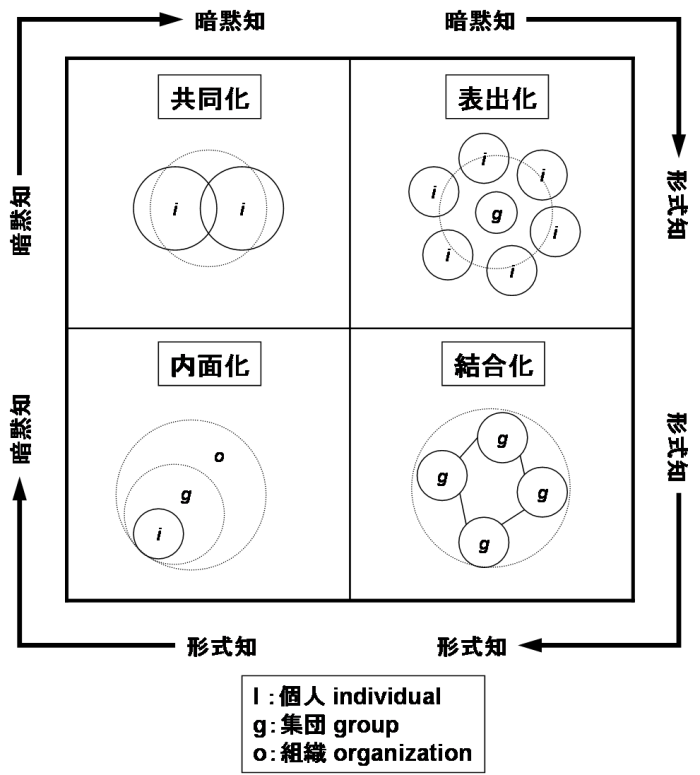
\includegraphics[width=15cm]{SECI_pro.PNG}
\caption{SECIプロセス}\label{サンプル図}
\end{figure}


\section{具体的な手法}
主に以下の手法があるが,それぞれ独立したものでなく,相互依存的なものである\cite{management}.
\subsection{データマイニング}
人工知能や統計学を利用してデータから知識を取り出そうとする試み.主に共起現象を探り,セールスに結びつけようとしている.

\begin{itemize}
  \item 例1:スーパーでビデオとガムが共に売れる→両者を同じ場所に置く.
  \item 例2:本Aを買う人は,後に本Bを買うことが多い→購入者に本Bを薦めるダイレクトメールを送る.
  \item 従来の統計学と大差ないが,POSやオンラインショッピングによる大量のITデータの中から法則性を見つけ出すことに主眼が置かれている\cite{management}.
\end{itemize}

\subsection{データウェアハウス}
データを多次元的に処理することにより,通常では察知しにくい傾向性を発見する技法.多次元データベースなど,幾つもの次元によって処理が可能なソフトウェアが開発されている.

\begin{itemize}
  \item 例:時間,空間,取り扱い物によって販売量が明示される → 時系列や地域、取り扱い物の傾向が分かる\cite{management}.
\end{itemize}

\subsection{知識共有化}
電子掲示板やメーリングリスト,知識ベース,オンラインコラボレーションなどを使って,一部の人の資産であった知識の,集団全体への共有を図るもの.
基本的には文字や印刷といったメディアの問題であるが,電子通信技術の一新によって,電子メール・電子掲示板に代表されるような新しい共有化のあり方が模索されている.
具体的には,企業内ではグループウェアなどを使って知識共有の試みが行われることが多い.インターネット上でも,OKWave,はてなのように広範な分野を扱うサイトや,Apple Support Discussionのような特定者向けサイトによる知識共有化の試みが始まっている.
近年,エンタープライズ2.0と呼ばれる大企業での情報共有が積極的に行われるようになってきた\cite{management}.


\subsection{可視化}
人間における視覚の優位性を利用し,多次元・多要素で理解しにくい情報を,見える形で表現し,理解しやすくさせること.
原理的にはグラフや図画であるが,ナレッジマネジメントではCGを利用した立体的で動的な画像を使って表現するケースが多い.


様々な手法はあるものの,通常の技法と同じく,それを使いこなすのは熟練と才能が必要とされるため,電子メールやQA知識ベースなどいくつかを除けば,実際に有効活用されている例は少ない.
また暗黙知を明示化するには原理的に大きな困難が伴うため,共有化された知識はあまり役に立たない常識的なものがほとんどで,実際にほしい熟練した技能や知恵は掘り出せないことが多いため,研究自体は尻すぼみになっている\cite{management}.

\subsection{エンタープライズサーチ}
企業組織内の書類,人事,経営情報等を検索できるようにするためのシステム,またはそのコンセプトのこと\cite{management}.


\section{知識変換の「場」}
組織として,知識の創造,共有,活用,蓄積を活発化させるために,個々のナレッジを共有したり,共同でナレッジを創造したりするための結節点が必要となる.この結節点を,「場」と言う.豊かな知識創造・知識経営が出来るかどうか,「場」のデザインにかかってくる.「場」は,SECIモデルの各フェーズに沿って,4つのパターンに分けることができる\cite{ba}.


\subsection{創発場(Originating Ba)}
\begin{itemize}
  \item 共同化に対応
\end{itemize}

経験,思い,信念,考え方などの暗黙知を共有する場である\cite{ba}.

\subsection{対話場(Dialoguing Ba)}
\begin{itemize}
  \item 表出化に対応
\end{itemize}

各自が対話(ダイアローグ)を通じて暗黙知を言語化・概念化して形式知に変換するための場である\cite{ba}.

\subsection{システム場(Systemizing Ba)}
\begin{itemize}
  \item 結合化に対応
\end{itemize}

形式知を相互に移転・共有・編集・構築し,新たな体系の形式知へと統合する場である\cite{ba}.

\subsection{実践場(Exercising Ba)}
\begin{itemize}
  \item 内面化に対応
\end{itemize}

形式知を個々人の暗黙知へと身体化するための場である.ここでは,単なる形式知の伝達ではなく,形式知に束ねる形で何らかの経験的要素や人間的要素を提供することで暗黙知としての移転・発展を促すことができる.サービス業などで特に重要な場である\cite{ba}.

\begin{figure}[H]
\centering
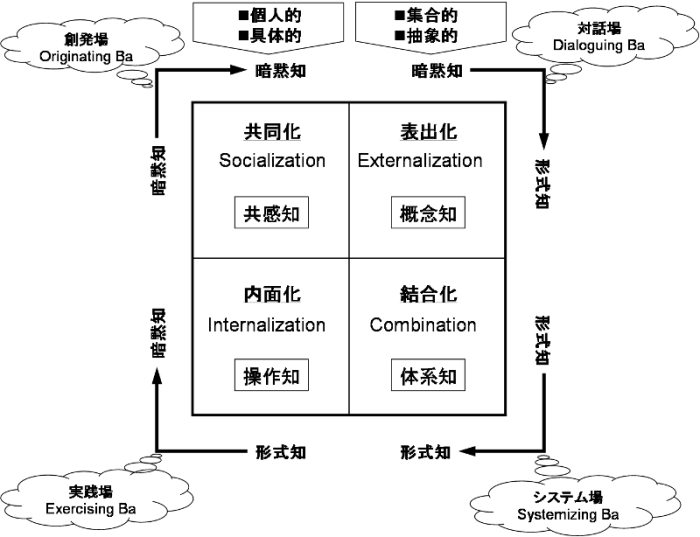
\includegraphics[width=15cm]{SECI_ba.PNG}
\caption{SECIプロセスの「場」について}\label{サンプル図}
\end{figure}

\chapter{株とは}
\section{株とは}
企業が事業資金を調達するために,発行しているものである.企業は,投資家が株を買ってくれた資金等を使って事業を拡大する.
「株を買う」ということは,株を発行している企業に出資を行い,事業資金を提供していることを意味する.

まとめると,株とは,
「株を買う(株主になる)」=「出資者になる」=「会社のオーナーの一人になる」
ことを意味する\cite{kaisya}.

また,株の大きな特徴として,買った株を第三者に転売することができる.株を転売すれば,会社のオーナー(株主)の権利等は,新しいオーナー(株主)に移ることになる\cite{kabu}.

\section{株式会社とは}
細分化された社員権(株式)を有する株主から有限責任の下に資金を調達して株主から委任を受けた経営者が事業を行い,利益を株主に配当する,法人格を有する企業形態である.このような企業形態は各国で見られる.

\section{株価変動の要因}
株価変動の要因はさまざまである.

上昇の要因と下落の要因を説明する.

\subsection{株価上昇の要因}
基本的に株が上がって行く状態というのは,買い手が多い,つまりはその株は人気が高い状態にあるよいうことである.
\begin{enumerate}
  \item 業績が好調である

業績が好調であるということは,利益を生み出しやすい状態にあるということである.投資家から人気が高いのは当然である.
  \item 業績の見通しを上方修正した

当初の会社の予想より,見通しを上方修正した時である.会社側が思っていたよりも利益が出そうという報告である.これも好感される.
 \item 復配・増配をする

今期は配当金を出す,または前回より配当金を増やすと発表した時である.復配や増配は,業績が好調の証であるため,投資家に好感されることがある.
  \item 新製品の発表・新しい工場の建設など

新しいことを始めるのは,リスクももちろんあるが,利益を増やすために行うものである.これにより利益が増えるという判断をされた場合には,株価が上がる.
  \item 合併・買収

企業の合併・買収により,企業間の相乗効果が出て,企業価値が上がると判断された場合には,株価が上がる.
  \item 割安株の修正

割安に放置されていた株が,とある出来事をきっかけに株価上昇が起きることがある.とある出来事というのは,上の1~5の理由もそうであるし,東証2部から東証1部へ移動することを発表し,
たくさんの投資家の目に触れたときにも株価が上がることがある\cite{kabuup}.
\end{enumerate}

\subsection{株価下落の要因}
 株価が下がるときは,株価が上がるときの要因の逆のことがおきたときである.基本的に株が下がって行く状態というのは,売り手が多い,つまりはその株は人気が低い状態にある.

\begin{enumerate}
  \item 業績が不調である

業績が不調であるということは,利益を生みにくい状態にあるわけである.投資家から人気が落ちるのは当然のことである.



  \item 業績の見通しを下方修正した

当初の会社予想より,見通しを下方修正した時である.会社側が思っていたよりも利益が少なそうという報告である.これも嫌気される.
 
  \item 無配・減配にする

今まで出していたが今期は配当金をださない,または前期より配当金を減らすと発表した時である.無敗や減配は,業績が不調の証であるから,投資家から嫌われる.

 
  \item 問題が起きる

経営トップの不祥事,工場の環境汚染,法律違反,事故の原因など悪い材料が明るみに出た場合である.
 
  \item 為替レート

円高・円安の影響を受ける企業がこれに当てはまる.特に輸出産業に関しては円高になると,製品の値段が実質的に上がってしまうため,利益が減るという意味で嫌気される.

  \item 同業他社の不振・倒産

同業他社が倒産すると,その業界自体が冷え込んでいる可能性がある.そういった思惑売りが出る.逆にその会社だけに問題がある場合は,売り上げアップのチャンスになるため,好感されることもある\cite{kabudown}.
\end{enumerate}

このように様々な理由で株価変動は起きるのである.





\chapter{研究方法}


チャレンジャー号墜落事故の事例と同じような条件の事故を調べる.



\section{調べる事故の条件}
\begin{itemize}
  \item 複数の企業が関わっていること
  \item 原因企業が判明するまでに時間がかかっていること
  \item 原因企業が株式会社であること

\end{itemize}


このような条件に当てはまる事故をウェブで検索して調べる.

\section{条件に当てはまる事故}
ウェブ検索で見つかった事故は以下の4件である.

\subsection{スペースシャトル・チャレンジャー号爆発事故}

1986年1月28日,アメリカ合衆国のスペース・シャトルチャレンジャー号が射ち上げから73秒後に分解し,7名の乗組員が死亡した事故である.同オービタは北米東部標準時午前11時39分(16:39UTC,1月29日1:39JST)にアメリカ合衆国フロリダ州中部沖の大西洋上で空中分解した.

<事故の概略>

機体全体の分解は,右側固体燃料補助ロケット(Solid Rocket Booster, SRB)の密閉用Oリングが発進時に破損したことから始まった.Oリングの破損によってそれが密閉していたSRB接続部から漏洩が生じ,固体ロケットエンジンが発生する高温・高圧の燃焼ガスが噴き出して隣接するSRB接続部材と外部燃料タンク(External Tank, ET)に悪影響を与えた.この結果,右側SRBの尾部接続部分が分離すると共に外部燃料タンクの構造破壊が生じた.空気力学的な負荷により軌道船は一瞬の内に破壊された\cite{bakuhatuziko}.

\begin{figure}[H]
\centering
\includegraphics[width=15cm]{challenger_explosion.PNG}
\caption{チャレンジャー号爆発」}\label{サンプル図}
\end{figure}


\subsection{トルコ航空DC-10パリ墜落事故}

1974年にフランスで発生したトルコ航空981便のDC-10-10(マクドネルダグラス社製,機体記号TC-JAV)が墜落した航空事故である(別名:トルコ航空981便墜落事故).

<事故の概略>

事故機は離陸10分後,,パリから北へ15km離れたサン=パトゥス村 (Saint-Pathus) 上空、高度11500フィート(3500メートル)まで上昇したときに,ロックが不完全だった左側後部貨物室ドアが客室の与圧により吹き飛ばされて急減圧が起こった.この時にパイロットが持っていたマニュアルが壁にたたきつけられる音がコックピットボイスレコーダーに収録されている.貨物室の減圧に伴い客室の床が破壊され,乗客6名が座席ごと空中に放り出された.また,床下を通るコントロールラインが切断されて,方向舵,昇降舵,尾部エンジンの制御が不可能になり,操縦不能のままドアの脱落から1分17秒後に430ノット(約796km/h)の速さで墜落に至った\cite{toruko}.


\begin{figure}[H]
\centering
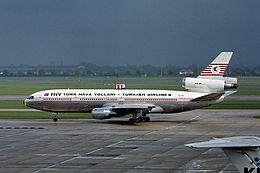
\includegraphics[width=15cm]{260px-McDonnell_Douglas_DC-10-10,_Turkish_Airlines_AN1815013.PNG}
\caption{トルコ航空DC-10」}\label{サンプル図}
\end{figure}


\subsection{日本航空123便墜落事故}

1985年(昭和60年)8月12日月曜日18時56分に,東京(羽田)発大阪(伊丹)行同社定期123便ボーイング747SR-100(ジャンボジェット,機体記号JA8119,製造番号20783)が,群馬県多野郡上野村の高天原山の尾根(通称「御巣鷹の尾根」)に墜落した航空事故である.

<事故の概略>      

事故機の後部圧力隔壁が損壊し,その損壊部分から客室内の空気が機体後部に流出したことによって,機体尾部と垂直尾翼の破壊が起こった.さらに、4系統ある油圧パイプがすべて破壊されたことで作動油が流出し,操縦機能の喪失が起こった\cite{nihon}.

\begin{figure}[H]
\centering
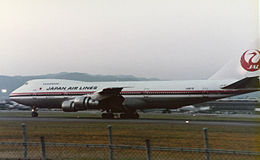
\includegraphics[width=15cm]{JA8119_at_Itami_Airport_1984.PNG}
\caption{日本航空123便」}\label{サンプル図}
\end{figure}


\subsection{東京航空交通管制システム障害}

2003年3月1日7時ごろ,飛行計画情報処理システム(FDP)のシステムトラブルは,航空会社の欠航便205便,30分以上の遅延便は1462便,また2日間にわたってダイヤが乱れるという大障害となった.

<障害の概略>
 
2002年9月に変更したFDPにNEC(日本電気(株))によるプログラム・ミスがあった.
2003年3月1日,「防衛庁システム対応プログラム」を変更したことと,当日7時,オンライン情報処理プログラムが起動したことにより,これまで隠れていたこのミスが表に現れ,システムがダウンした\cite{kouku}.


\section{事故当日の株価変動データの取得}

原因企業と関連する企業の事故当日の株価データを調べる.
原因企業に関連するの企業の株価も大幅下がっていたら,
それは研究背景の内容とは異なってくるためである.

原因企業以外の株価を調査するため,その事故当日の株価の変動データを『Rubyによるクローラー開発技法』を参考にして,コードを入力し,
株価変動データを取得する\cite{miyake}.

\begin{figure}[H]
\centering
\includegraphics[width=15cm]{ruby.PNG}
\caption{『Rubyによるクローラー開発技法』}\label{サンプル図}
\end{figure}

その中でその日に下がっている株価を抽出し,事故に関連性のある企業があるかかないかを調べる.
さらに関連性のある企業を抽出したら,その企業が事故にどの程度関与しているのかを調べ,株式市場は賢かったのか,チャレンジャー号墜落事故の事例は偶然であったのかを判断する.



\chapter{Rubyによるクローラー開発}
\section{クローラーとは}
クローラーとはシステムが自動的にWebページを巡回して情報を収集するプログラムである.クローラーとしてもっとも有名なのは,Googleなどの検索エンジンである\cite{miyake}.

\section{Rubyとは}
Rubyは1993年から開発されている国産オブジェクト指向スクリプト言語である.代表的な汎用スクリプト言語Rerlに可読性の高い構文とシンプルかつ強力なオブジェクト指向を加え,Lisp風の味付けをしたものがRubyである\cite{miyake}.

                                                                                         


\chapter{結果}
\section{各事故の原因企業}
\subsection{スペースシャトル・チャレンジャー号爆発事故}
原因企業:モートン=サイオコール社

※現在:ATKランチ・システムズ・グループ英: ATK (Launch Systems Group)  

ATKランチ・システムズ・グループ(英: ATK Launch Systems Group)は,初期にはゴム及び関連した化学製品に携わり,後にロケットとミサイルの推進システムに携わるアメリカ合衆国の企業である.ATKとは親会社のアライアント・テックシステムズ (Alliant Techsystems Inc.)の略(NYSEコード)である.

2006年に現在の社名になるまで.社名は一定ではなかったものの常にThiokolの名が入っていた.Thiokolは,同社の最初の製品のポリサルファイド系ポリマーの商品名で,ギリシア語で硫黄を意味するtheioと接着剤を意味するkollaの混成語である\cite{saiokoru}.
\subsection{トルコ航空DC-10パリ墜落事故}
原因企業:マクドネル・ダグラス社

民間や軍用の数多くの著名な飛行機を生産している.ジェームズ・スミス・マクドネル(James Smith McDonnell)設立のマクドネル・エアクラフト社とドナルド・ウィルズ・ダグラス(Donald Wills Douglas)設立のダグラス・エアクラフト社の合併により1967年に誕生した.カリフォルニア州ロングビーチとミズーリ州セントルイスに製造工場がある.1997年にボーイング社に吸収合併された\cite{dagurasu}.
\subsection{日本航空123便墜落事故}
原因企業:ボーイング社

ボーイング(The Boeing Company)は,アメリカ合衆国に所在する世界最大の航空宇宙機器開発製造会社.1997年にマクドネル・ダグラス社を買収したため,現在アメリカで唯一の大型旅客機メーカーであり,ヨーロッパのエアバスと世界市場を二分する巨大企業である.また民間機だけでなく,軍用機,ミサイル,宇宙船や宇宙機器などの研究開発・設計製造を行う.機体の設計に関して,有限要素法の設計手法の導入に先んじていて,その技術は車輌構体設計など他分野にも技術供与されており,世界の航空宇宙機器業界をリードしている\cite{boing}.
\subsection{東京航空交通管制システム障害}
原因企業:日本電気株式会社

日本電気株式会社(にっぽんでんき,英:NEC Corporation,略称:NEC(エヌ・イー・シー),旧英社名 Nippon Electric Company, Limitedの略)は,東京都港区芝五丁目(元・東京都港区芝三田四国町)に本社を置く住友グループの電機メーカー.大手電機8社の一角(日立製作所,パナソニック,東芝,三菱電機,ソニー,シャープ,日本電気,富士通).
日電(にちでん)と略されることも稀にあるが,一般的には略称のNECが使われ,ロゴマークや関連会社の名前などにもNECが用いられている\cite{nihondenki}.
\chapter{考察}

\chapter{結論}





\bibliographystyle{junsrt}
\bibliography{biblio}%「biblio.bib」というファイルが必要.

\end{document}
